\chapter{Methodology}\label{chapter:methodology}

% \begin{rawidea}
% The vehicle parameter ranges were considered as variations to the baseline combination. While some OEM limitations may not allow for certain ranges of a parameter, there is a possibility that with new technologies and manufacturing modularity that such variations may become available. Thus it is important to note what can be changed as a whole for the combination that is being looked at when attempting to optimise the design.
% \end{rawidea}

% \begin{rawidea}
% To simplify the geometry, the dimensions of the baselines in the case of overhangs were assumed as boxes. This is generally true of trailer structures, however the prime movers are more stylistic and rounded. Thus narrower values for overall width of the prime mover were investigated.
% \end{rawidea}

% \begin{rawidea}
% The rear overhang reported was with respect to the last axle in the axle group to align with the definition from the \gls{nrta} for maximum rear overhang.
% \end{rawidea}

% \begin{rawidea}
% Each parameter was altered in isolation, thus the interaction with the other baseline parameters needed to be considered in order to ensure stable dynamic models.
% \end{rawidea}

% \begin{rawidea}
% While it was not a requirement that the combinations simulated were legal within prescriptive legislation, the legislation was used as a guide to generate reasonable vehicle design parameters to avoid instability in the model
% \end{rawidea}

The study of the relative effect of the \glspl{vdp} of \glspl{hcv} was split into three parts:

\begin{enumerate}
	\item Develop a set of three baseline combinations that represent a range of highly productive heavy vehicles. Previous \gls{pbs} assessments conducted by \gls{wits} and the \gls{csir} were used.
	\item Define reasonable ranges for each \gls{vdp} by considering \gls{oem} variations, legal restrictions, physical constraints, and data from \gls{pbs} assessments previously conducted by Wits.
	\item Evaluate the relative effect of altering each \gls{vdp} on overall vehicle performance within the \gls{pbs} framework as detailed explained in Section~\ref{section:interpretation-of-the-results-matrix}.
\end{enumerate}

\trucksim{} was used as the multi-body vehicle dynamics simulation package to simulate the \gls{pbs} manoeuvres. The simulation results were used to determine the safety of each \gls{hcv} within the \gls{pbs} framework using a post processor developed in \matlab{} at \gls{wits}. Software versions and descriptions are included in Section~\ref{section:software}.

A \matlab{} script automated the adjustment of each individual or combination of parameters within a \trucksim{} model according to the work flow illustrated in Figure~\ref{figure:matlab-trucksim-api-interaction} allowing for the simulation of a large set of vehicle configurations.

The simulation models and method were validated using results published by the \gls{ntc} as presented in Section~\ref{section:validation-method}.

%----------------------------------------------
%      FIGURE
%----------------------------------------------
\begin{figure}[H]
	\centering
	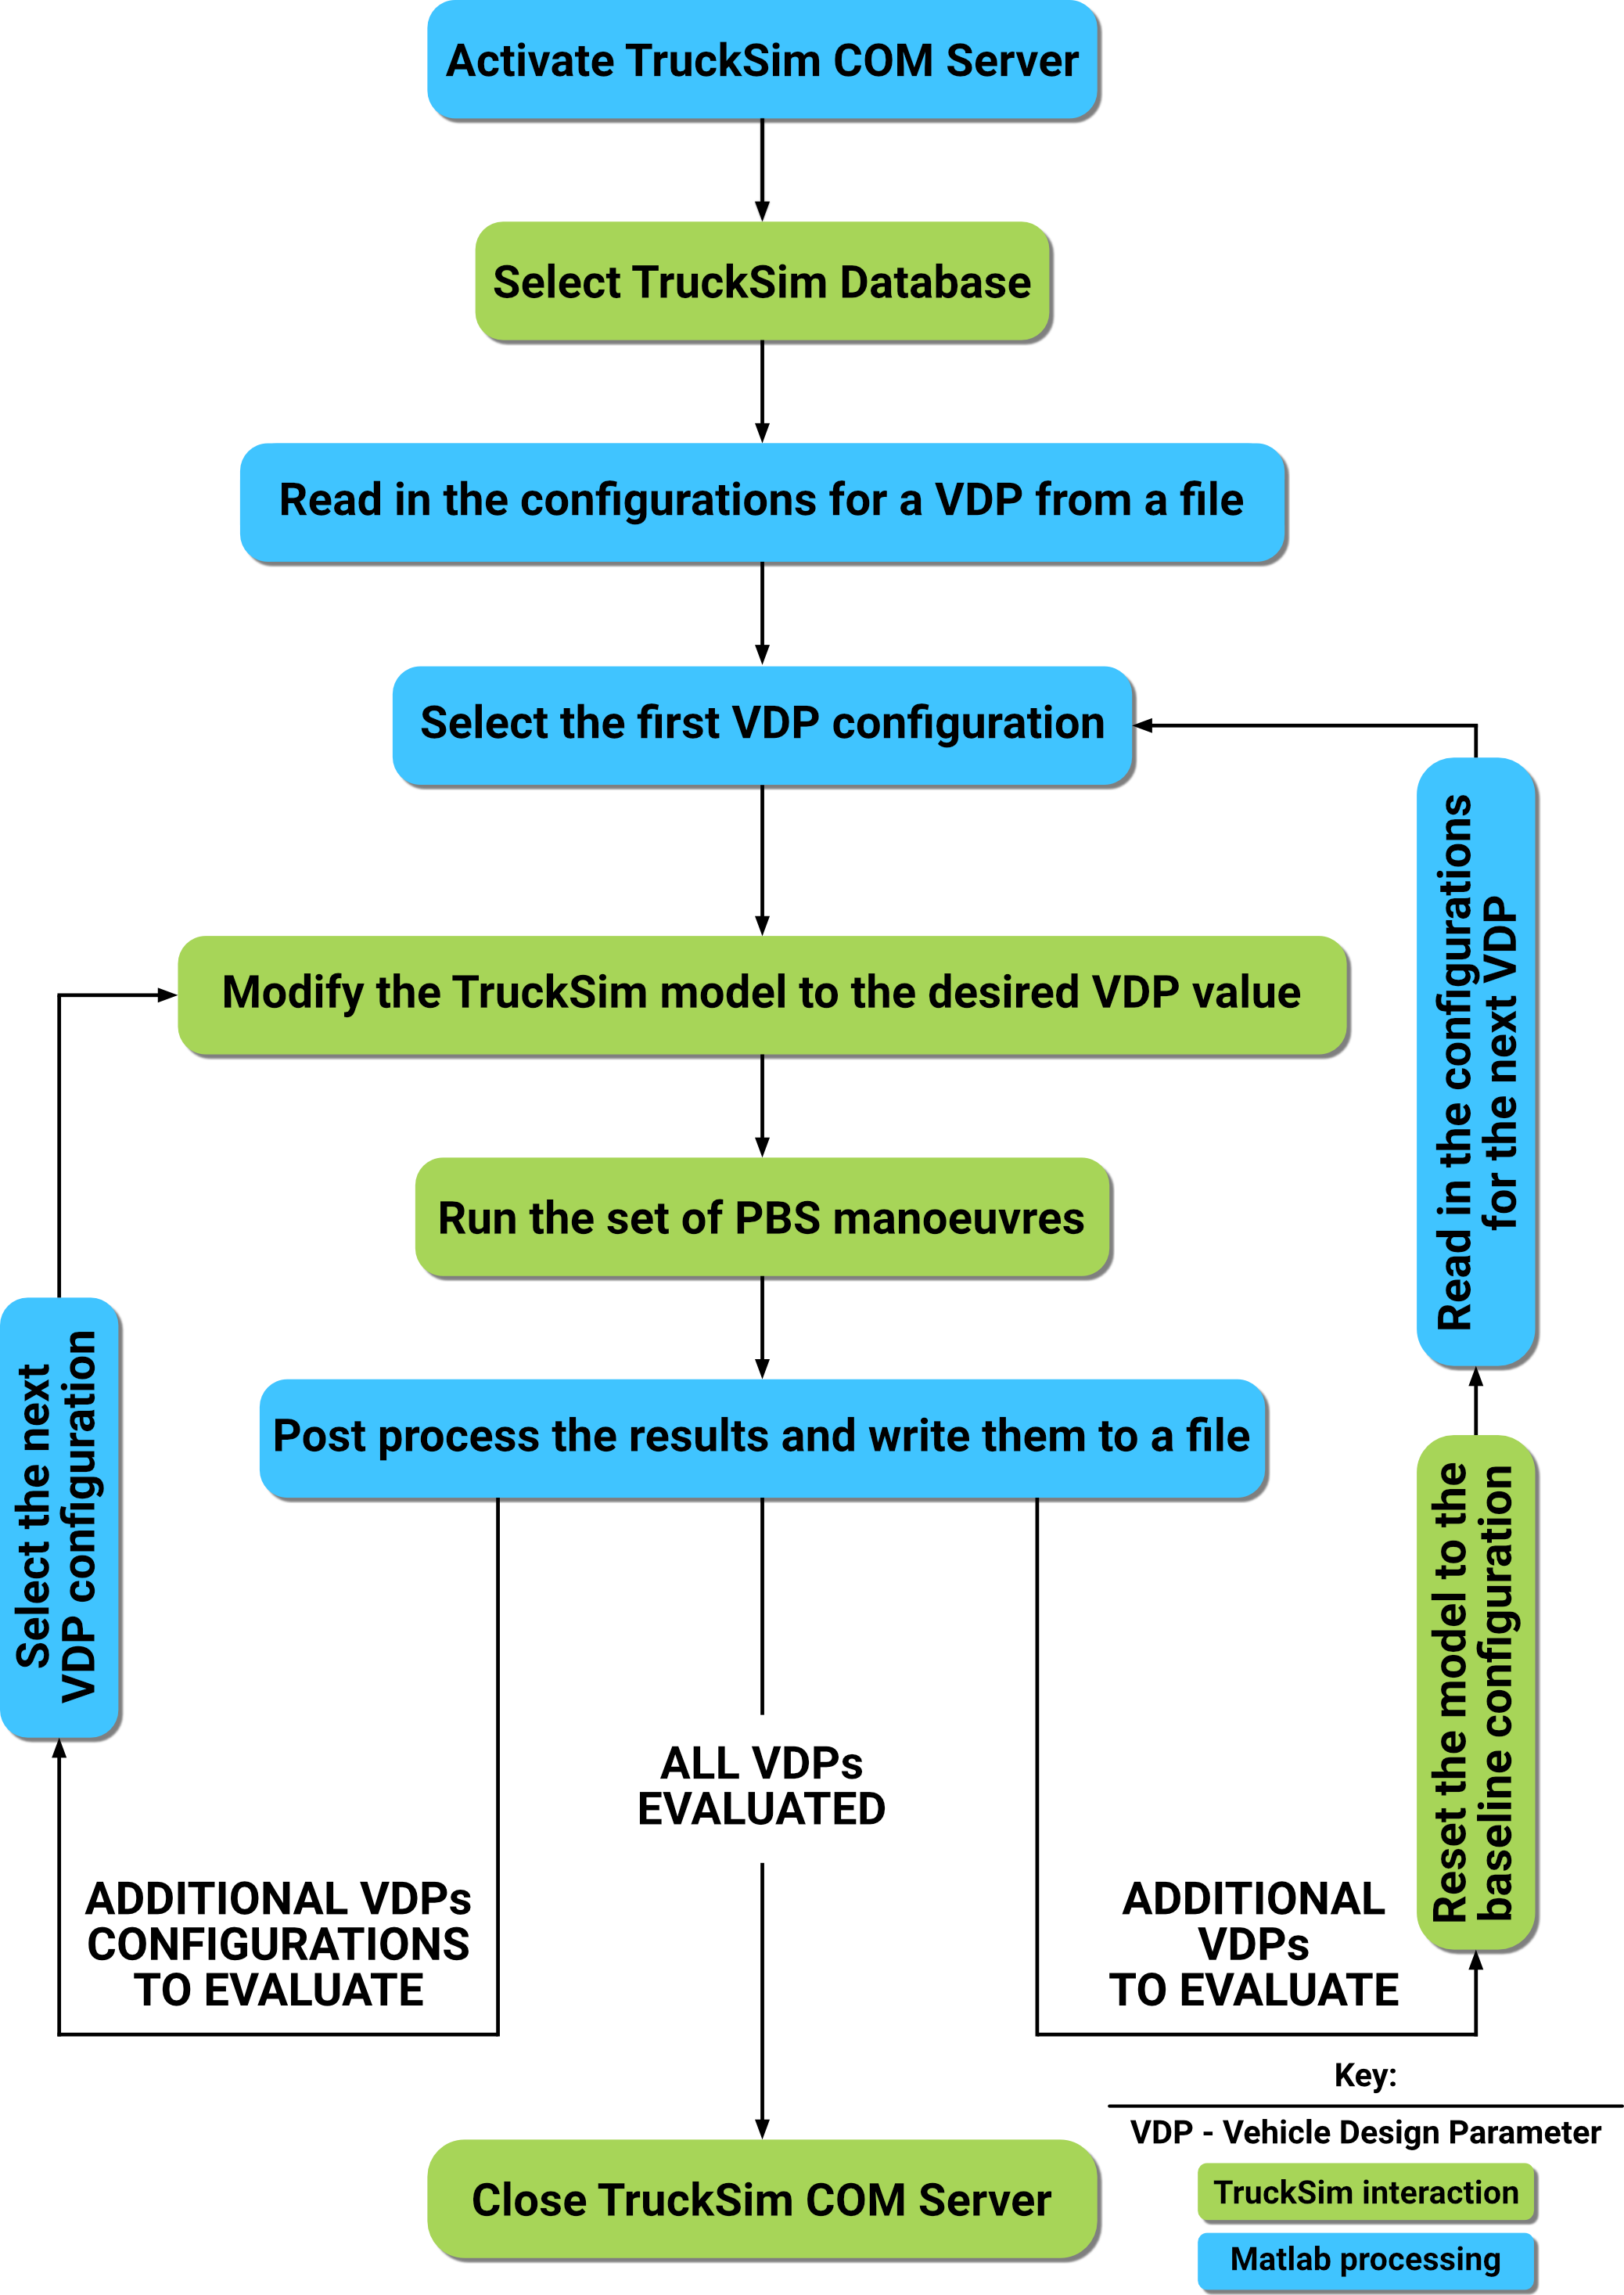
\includegraphics[width=1\textwidth]{fig/2018-03-23_trucksim-com-server-flowchart}
	\caption{\matlab{} interaction with the \trucksim{} 2018 API using a COM server}
	\label{figure:matlab-trucksim-api-interaction}
\end{figure}
%----------------------------------------------
%      FIGURE
%----------------------------------------------

%==============================================
%      SECTION
%==============================================
\section{Software}\label{section:software}

The following software packages were used to perform the vehicle simulations:

\begin{enumerate}
	\item \textbf{\trucksim{} 2018 \cite{MechanicalSimulation2016}:} a multi-body vehicle dynamics package used to simulate the various \gls{hcv} vehicle configurations performing the \gls{pbs} manoeuvres.
	\item \textbf{\matlab{} 2018 \cite{MATHWORKS2015}:} a high-level coding environment capable of performing numerical computation and visualisation. Matlab was used in two ways; to post process the simulation outputs of the \trucksim{} simulations and determine vehicle performance within the \gls{pbs} framework and to compare the relative effect of each \gls{vdp} on vehicle performance.
\end{enumerate}

%==============================================
%      SECTION
%==============================================
\section{Validation Method}\label{section:validation-method}

The \gls{ntc} requested consultants to compare three computer-based modelling packages (ADAMS, AUTOSIM and \glspl{umtri} Yaw/Roll) to evaluate (in isolation of each other) the \gls{pbs} performance of a B-double and truck-trailer heavy vehicle combination \cite{Prem2001} (known as an interlink and rigid drawbar combination in South Africa).

The \gls{ntc} prescribed a set of inputs for a representative B-double and truck-trailer combination used by all consultants. The vehicles were simulated to perform identical pulse steer, step steer, standard SAE lane change and a low-speed 90\degree{} turn manoeuvres.

The B-double was found to have excellent agreement between all three of the modelling packages. The truck-trailer combination is an inherently less stable vehicle and produced larger but still acceptable amounts of variation in results between the modelling packages.

The Yaw/Roll simulation results were provided by the \gls{ntc} for service providers to calibrate their computer-modelling software and techniques. This data was used to validate the models.

\subsection{Validation Results}\label{section:validation-results}

The behaviour of the B-double and truck-trailer simulated in \trucksim{} 2018 was found to have good correlation with the behaviour simulated in \glspl{umtri} yaw/roll program. Similarly to the outcome of the \gls{ntc} validation, the truck-trailer combination compared less favourably than the B-double combination due to it being a less stable configuration.

Differences in simulated behaviour are attributed to improvements to the prediction of heavy vehicle performance with the latest solvers, differences in the driver models and additional degrees of freedom in the \trucksim{} modelling package.

A set of graphs comparing the simulated vehicle behaviour in \trucksim{} 2018 and \glspl{umtri} yaw/roll program are included in Appendix~\ref{appendix:NTC-validation}.